\normaltrue \difficilefalse \tdifficilefalse
\correctionfalse

%\UPSTIidClasse{12} % 11 sup, 12 spé
%\newcommand{\UPSTIidClasse}{12}

\exer{Pompe à palettes  $\star$ \label{TEC:05:C2:09:10}}
\setcounter{question}{0}\marginnote{\xpComp{TEC}{05}}%\UPSTIcompetence[2]{C2-09}
\index{Compétence C2-09}\index{Compétence TEC-05}
\index{TEC}
\index{Théorème de l'énergie cinétique}
\index{Pompe à palettes}
\ifcorrection
\else
\marginnote{\textbf{Pas de corrigé pour cet exercice.}}
\fi

\ifprof
\else
Soit le mécanisme suivant. On a $\vect{AO}=e\vect{i_0}$ et $\vect{AB}=\lambda(t)\vect{i_1}$. De plus $e=\SI{10}{mm}$ et $R=\SI{20}{mm}$. Le contact entre \textbf{0} et \textbf{2} en $B$ est maintenu en permanence (notamment par effet centrifuge lors de la rotation de la pompe). De plus, on note :
\begin{itemize}
\item $G_1 = A$ le centre d'inertie du solide \textbf{1}, $m_1$ sa masse et $\inertie{G_1}{1}=\matinertie{A_1}{B_1}{C_1}{0}{0}{0}{\rep{1}}$ sa matrice d'inertie;
\item $G_2$ le centre d'inertie du solide \textbf{2} tel que $\vect{BG_2}=-\ell \vi{1}$, $m_2$ sa masse et $\inertie{G_2}{2}=\matinertie{A_2}{B_2}{C_2}{0}{0}{0}{\rep{2}}$ sa matrice d'inertie.
\end{itemize}
On note $C_m\vk{0}$ le couple moteur agissant sur le solide \textbf{1}, $F_h\vi{1}$ l'action du fluide sur \textbf{2} (le fluide agissant sur les solides \textbf{1} et \textbf{2}).  L'accélération de la pesanteur est donnée par $\vect{g}=-g\vj{0}$.

\begin{marginfigure}
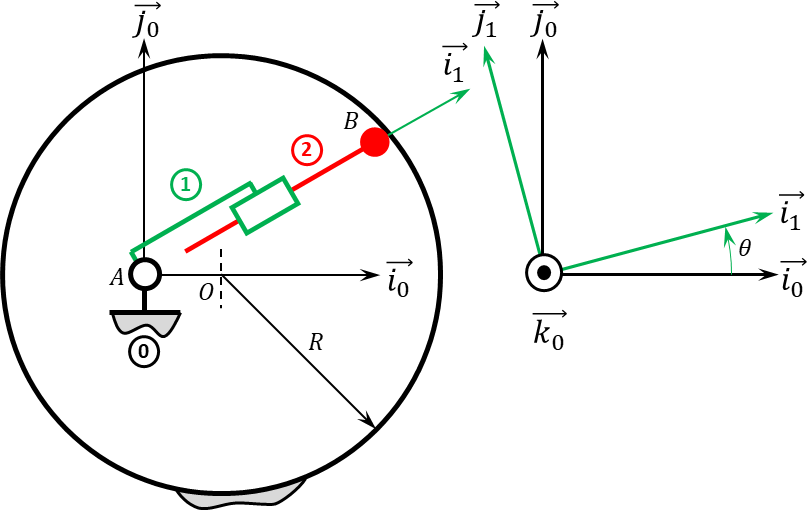
\includegraphics[width=\linewidth]{10_01}
\end{marginfigure}
\fi

On rappelle que la loi entrée sortie est donnée par la relation *** établie à l'exercice \ref{C2:06:10}.

\question{Tracer le graphe d'analyse en indiquant l'ensemble des actions mécaniques agissant sur les différents solides.}
\ifprof
\else
\fi

\question{Déterminer l'ensemble des puissances intérieures à l'ensemble \textbf{1+2}.}
\ifprof
\else
\fi

\question{Déterminer l'ensemble des puissances extérieures à l'ensemble \textbf{1+2}.}
\ifprof
\else
\fi

\question{Déterminer $\ec{1+2}{0}$.}
\ifprof
\else
\fi

\question{Déterminer la loi de mouvement en appliquant le théorème de l'énergie cinétique.}
\ifprof
\else
\fi


\ifprof
\else

\marginnote{Corrigé  voir \ref{TEC:05:C2:09:10}.}

\fi